\chapter{Metastability and phononic CDW quench in \ce{TaTe2}}
\label{ch:tate2}

Collective phenomena arising from complex many-body interactions have been a focal point in condensed matter physics for several decades.
A prominent example is the charge density wave (CDW), a collective ordering of electron-hole pairs, first introduced by Peierls in 1955 \cite{peierls_quantum_1996}.
Since its inception, the concept of CDWs has been intricately linked to superconductivity \cite{frohlich_theory_1997}.
The relevance of CDWs gained momentum when experimental evidence began to emerge in the first materials hosting such exotic phases, decades after the original theoretical proposal.
Early experimental observations came from pioneering studies on blue bronzes by Fogle and Perlstein \cite{fogle_semiconductor--metal_1972} and transition metal trichalcogenides by Monceau \cite{monceau_electric_1976}.

Over the following decade, a wide range of systems were found to exhibit CDW phases, leading to an intense research focus on understanding these phenomena, as reflected in numerous publications and reviews during that period \cite{wilson_questions_1978,gruner_dynamics_1988,yoffe_electronic_1990,wilson_charge-density_2001}.
Among these, transition metal chalcogenides garnered particular attention due to their rich phase diagrams and layered structures.
The layered nature of these materials was recognized early on in transition metal dichalcogenide (TMD), with exfoliation of \ce{MoS2} demonstrated in 1963 \cite{frindt_physical_1997}, and monolayer samples achieved by 1986 \cite{joensen_single-layer_1986}.
Concurrently, research on graphite led to the creation of graphene monolayers, sparking a surge of interest in layer engineering across materials like graphene, \ce{WS2}, and \ce{MoS2} \cite{iijima_helical_1991,tenne_polyhedral_1992,feldman_high-rate_1995}

The complexity of these materials stems from their strongly correlated many-body nature, leading to intricate phase diagrams and making it difficult to predict and understand their properties.
Since the 1980s, CDW research in TMDs has largely focused on the \ce{TaX2}-based compounds \ce{TaS2} and \ce{TaSe2}, with their diverse phase diagrams, which include multiple CDW phases as well as superconducting states.
These phase transitions are fairly well understood within the classical Peierls framework.
Recent studies have demonstrated that phase transitions in \ce{TaS2} can be triggered by light or electrical pulses, resulting in metastable hidden states \cite{vaskivskyi_controlling_2015,maklar_coherent_2023}.
The ability to modify electronic properties on ultrafast timescales, combined with the stability of these hidden states, has opened avenues for potential applications in switches and memory devices.

Despite the significant attention on \ce{TaS2} and \ce{TaSe2}, the sister compound \ce{TaTe2} has remained relatively underexplored.
However, recent studies have begun to investigate this material, particularly due to its unusual behavior during the CDW phase transition, which differs from its sister-compounds.

In this chapter, I will present both static and time-resolved ARPES (trARPES) data on \ce{TaTe2}, with the goal of exploring the driving mechanisms behind CDW formation and the associated structural phase transition.
First, I will introduce the general concept of CDWs in 1D systems and the challenges that arise in higher dimensions and with strong coupling.
I will then review CDW behavior in \ce{TaX2} compounds.
Following that, I will examine the band structure and Fermi surface topology of \ce{TaTe2}, comparing the material's high- and low-temperature phases, and discuss the formation of CDW-induced minigaps, first observed by Lin et al. \cite{lin_evidence_2022}.
Next, I will describe the ultrafast charge dynamics occurring on a few-picosecond timescale, including the delayed melting of the CDW.
This femtosecond-scale light excitation is accompanied by strong, band-specific oscillations, which will be analyzed in terms of their frequency, energy, and momentum-resolved coupling between phonons and electrons.
Lastly, I will present evidence of a metastable electronic state persisting for more than \qty{200}{\pico\second} and discuss its relevance to the structural phase transition at equilibrium.

\section{Charge Density Waves in strongly correlated matter}
\label{sec:cdw}

Charge density waves (CDWs) represent a collective modulation of the electron density, where electron-hole pairs can form and condense and behave as a macroscopic quantum state.
These waves are typically accompanied by a periodic lattice distortion (PLD) due to the coupling between electrons and phonons.
The concept of CDWs and PLDs was first introduced by Peierls in 1955 in the context of a 1D atomic chain \cite{peierls_quantum_1996}.
Since then, significant effort has been dedicated to understanding CDWs at a microscopic level, particularly in one-dimensional (1D) systems, where the theory is well established. However, when the dimensionality increases or strong coupling is involved, the descriptions become elusive, and these cases remain an active area of research.

In this section, I will briefly review Peierls' description of 1D CDWs and then introduce the challenges that arise when extending the theory to higher dimensions and strong coupling, with a focus on transition metal dichalcogenides (TMDs).
The foundation for this section is based on recent reviews of CDWs in TMDs \cite{rossnagel_origin_2011, canadell_importance_1992}.


\begin{figure}[t]
	\centering
	\begin{subfigure}[b]{0.45\textwidth}
		\includegraphics[width=\textwidth]{tate2/lindhard.png}
	\end{subfigure}
	\hfill
	\begin{subfigure}[b]{0.5\textwidth}
		\includegraphics[width=\textwidth]{tate2/nesting_sketch.pdf}
	\end{subfigure}
	\\
	\begin{subfigure}[b]{0.9\textwidth}
		\includegraphics[width=\textwidth]{tate2/pld_cdw_sketch_mod.pdf}
	\end{subfigure}
	\caption{(a) 1T' RT phase of \ce{TaTe2} forming ribbons. (b) 1T" LT phase of \ce{TaTe2}, \ce{Ta} atoms move together forming heptameres. (c) Resistivity of \ce{TaTe2} as a function of temperature with an overall reduction in resistivity while cooling. A phase transition occurs at \qty{170}{\kelvin}, which is accompanied by a further steplike reduction in resistivity.}
	\label{fig:cdw_theory}
\end{figure}

Starting from the 1D atomic chain of a metal with a lattice spacing $a$, a cosinusoidally modulated electron density can be described by
\begin{equation}
	\rho(\mathbf{r}) = \rho_0(\mathbf{r})[1+\rho_1 \cos(\mathbf{q}_0\mathbf{r}+\phi)]
	\label{eq:cdw}
\end{equation}
where $\rho_0$ is the unperturbed electron density, $\rho_1$ is the modulation amplitude, $\mathbf{q}_0$ the wavevector and $\phi$ the phase of the electron density modulation.
The term $\rho_1 \cos(\mathbf{q}_0\mathbf{r}+\phi)$ describes a standing wave of charge density with a wavelength of $\lambda_0 = 2\pi/\lvert \mathbf{q}_0\rvert$.
This modulation of the charges as a function of $\mathbf{r}$ creates an effective potential, felt by the underlying ionic atom cores, resulting in the ions moving away from their respective equilibrium position, to accommodate this new modulated potential.
The result is a distorted lattice, which is referred to as a periodic lattice distortion (PLD), and is of the form
\begin{equation}
	u_n = u_0 \sin(n\lvert \mathbf{q}_0\rvert a+\phi).
	\label{eq:pld}
\end{equation}
In this equation, $u_n$ is the atom position, $n$ describes the atom and $u_0$ the amplitude of the distortion.
Figure \ref{fig:cdw_theory} (c) illustrates the PLD and the corresponding CDW for a 1D atomic chain.

It is important to stress that while in our discussion we assume an existing electron modulation, resulting in a PLD, the reverse order of reasoning is also possible.
Namely a PLD will result in a corrugate CDW.
The pre-existing PLD generates a new effective potential that conduction electrons attempt to screen, leading to the formation of a modulated charge density, as described by Eq. \ref{eq:cdw}.
Thus, CDWs and PLDs are inherently interconnected and mutually reinforcing phenomena \cite{rossnagel_origin_2011, chan_spin_1973, johannes_fermi_2008}.

The transition to a 1D CDW state as described by Peierls relies on the fact that the material is described as a Fermi liquid, and the electron gas is only weakly coupled with the ions, for example in a weak electron-phonon coupling limit.
In a 1D system the Fermi surface consists of parallel sheets situated at momenta $+k_f$ and $-k_f$ (see Fig. \ref{fig:cdw_theory} (b)).
The connection of electrons with different Fermi momenta creates an instability at the Fermi surface, which leads to a divergence of the electron-hole lindhard response function.
In the presence of a finite electron-phonon coupling the system becomes unstable, which drives a structural phase transition.
This coupling of electrons with Fermi velocities of opposite signs via a wavevector of equal amplitude is called Fermi surface nesting (FSN)
Since the CDW formation and the FSN depend on the Fermi momenta ($k_f$), the CDW necessarily depends on the conduction band filling.
Additionally, the potential created by the CDW and PLD results in a gap opening at the Fermi level.
This potential is, for a given phonon mode $\mathbf{q}$ with the corresponding displacement $u_\mathbf{q}$, defined by
\begin{equation}
	v_\mathbf{q} = g_\mathbf{q} u_\mathbf{q} \sqrt{\frac{2M\omega_\mathbf{q}}{\hbar}}
\end{equation}
with the electron-phonon coupling $g_\mathbf{q}$ and the mass of the ion $M$.
Opening a gap at $E_F$ clearly lowers the energy of the occupied states while simultaneously increasing the energy of the unoccupied part of the band structure.
The energy change due to the gap opening caused by the potential $v_\mathbf{q}$ amounts to
\begin{equation}
	\delta E_\text{band} = -\lvert v_\mathbf{q}\rvert^2 \chi_0(\mathbf{q})
\end{equation}
with the non-interacting electronic susceptibility
\begin{equation}
	\chi_0(\mathbf{q}) = \frac{1}{L} \sum_{k}^{} \frac{f_{\mathbf{k}+\mathbf{q}}-f_\mathbf{k}}{\epsilon_\mathbf{k}-\epsilon_{\mathbf{k}+\mathbf{q}}}>0
	\label{eq:susz}
\end{equation}
$\chi_0$ represents therefore the net energy gain of the gapped band, and is dependent on the length of the atomic chain $L$ and the Fermi function $f(\epsilon_k)$ of the two nested states.
If the energy gain of the band exceeds the energy cost of the  strained lattice, which is given by
\begin{equation}
	\delta E_\text{lattice} = \frac{1}{2} M\omega_\mathbf{q}^2 u_\mathbf{q}^2
\end{equation}
than the CDW and PLD are the new ground state of the system.

With the above equations in mind, and by including Coulomb $U_\mathbf{q}$ and exchange interactions $V_\mathbf{q}$, it is possible to formulate a criterion \cite{chan_spin_1973}.
\begin{equation}
	\frac{4g_\mathbf{q}^2}{\hbar\omega_\mathbf{q}}-2U_\mathbf{q}+V_\mathbf{q}\geq\frac{1}{\chi_0(\mathbf{q})},
\end{equation}
for which a CDW state is formed.
This criterion indicates, that strong electron-phonon coupling $g_\mathbf{q}$, small Coulomb interaction, strong exchange interaction $V_\mathbf{q}$, small lattice strain energy $\omega_\mathbf{q}$ and a large $\chi_0(\mathbf{q})$ are the ingredients to form a CDW state.
The magnitude of aforementioned gap can be calculated by looking at the splitting of the normal-state band $\epsilon_\mathbf{k}$, assuming a tight-binding dispersion $\epsilon_\mathbf{k}=-E_F\cos(ka)$.
The splitting of the band occurs due to the fact, that the PLD superstructure wavevector $\mathbf{q}_0$ is equal to Fermi points $\pm\mathbf{k}_F$, which describe the Fermi nesting condition, which describes a energy discontinuity and the split band can be described by
\begin{equation}
	E_{1,2}(\mathbf{k})=\frac{\epsilon_{\mathbf{k}}+\epsilon_{\mathbf{k}+\mathbf{q}_0}}{2}\pm\sqrt{\left( \frac{\epsilon_{\mathbf{k}}+\epsilon_{\mathbf{k}+\mathbf{q}_0}}{2}\right)^2 + \Delta^2 }.
	\label{eq:cdw_splitting}
\end{equation}
$2\Delta$ represents the magnitude of the energy gap, which depends on the displacement amplitude of the PLD, the electron-phonon coupling $g_{\mathbf{q}_0}$ and the phonon frequency $\omega_{\mathbf{q}_0}$ \cite{gruner_density_2019}, with
\begin{equation}
	\Delta=u_{\mathbf{q}_0} + g_{\mathbf{q}_0} \sqrt{\frac{2M\omega_{\mathbf{q}_0}}{\hbar}}.
\end{equation}

As has been mentioned throughout this section, the CDW ground state occurs usually due to the presence of strong electron-phonon coupling.
The previous equation \ref{eq:cdw_splitting} already indicated the modifications to the electron dispersion due to the presence of this CDW state.
But, assuming the presence of strong electron-phonon coupling, a significant modification to the phonon dispersion is expected as well.
This change can be identified by first considering the temperature dependent Lindhard response function, within a similar tight binding picture as previously done for the modification to the electronic band strucutre.
The temperature dependent Lindhard response function at a wavevektor $\mathbf{q}=2k_F$ can be expressed as
\begin{equation}
	\chi_0 (2\mathbf{k}_F, T)=\frac{1}{2}\text{DOS}(E_F)\ln\left( \frac{2.28E_F}{k_BT}\right)
\end{equation}
with the density of states DOS$(E_F)$ at the Fermi level of the normal state.
Considering a large $E_F/k_BT$, the susceptibility will diverge when $T$ is lowered.
The divergence in the temperature dependent susceptibility indicates a renormalization of the phonon frequency in a wavevector range around $\mathbf{q}_0$, and is typically referred to as a Kohn anomaly.
The renormalized phonon frequency can be expressed by
\begin{equation}
	\widetilde{\omega}_\mathbf{q}^2 = \omega_\mathbf{q}^2 \left( 1-\frac{4g_\mathbf{q}^2}{\hbar\omega_\mathbf{q}} \chi_0(\mathbf{q}) \right)
	\label{eq:kohn}
\end{equation}
which reaches $0$ at finite temperatures $T_0$, if the electron-phonon coupling constant $g_{\mathbf{q}_0}$ is non-zero, resulting in the full softening of the phonon mode.

The finite temperature at which the phonon completely softens corresponds to the transition temperature between normal- and CDW-state.
From the equation \ref{eq:kohn} expressing the Kohn anomaly and by minimizing the total energy change of band and lattice $\delta E_\text{band}+\delta E_\text{lattice}$, it can be shown that, at $T=0$, the gap fulfills the following equation
\begin{equation}
	\Delta(0)=4E_F\exp(-\frac{1}{\lambda}),
\end{equation}
with the electron-phonon coupling constant $\lambda=\frac{2g_{\mathbf{q}_0}^2DOS(E_F)}{\hbar\omega_{\mathbf{q}_0}}$ \cite{rice_theory_1973}.
From the above equation it is possible to calculate the relation between the energy gap at zero temperature and the transition temperature, which is known as the Bardeen-Cooper-Schrieffer (BCS) relation.
For $\lambda\lesssim1$, which depends on the material properties, the BCS relation can be expressed as
\begin{equation}
	2\Delta(0)=3.52k_BT_0.
\end{equation}

This description provides a comprehensive microscopic theory of CDW formation under the assumption of a non-interacting 1D metal.
However, it is important to note that these assumptions rarely hold for most materials.
The solution for the 1D chain, which predicts long-range order at a finite transition temperature $T_0$, is generally only applicable to quasi-1D systems.
In fact, a purely 1D atomic chain cannot maintain stable long-range order due to thermal and quantum fluctuations that lead to dephasing.
To stabilize the long-range order, collective interlayer motion is required.
Moreover, the Peierls instability at $E_F$ arises from the exclusion of electron-electron interactions, as represented by the non-interacting susceptibility $\chi_0$.
Once these interactions are included, a material might remain stable, even at very low temperatures, preventing the formation of a CDW.
In light of these considerations, I will further discuss the consequences of higher dimensionality and strong electron-phonon coupling on CDW formation, both of which are relevant in the case of \ce{TaTe2}.

To summarize, in a 1D system, CDW formation is driven by the instability of the non-interacting electronic susceptibility, resulting from the coupling of many electronic states by the same wavevector $\mathbf{q}$, with most of them located near $E_F$.
In such systems, the Fermi surface is planar, and the $\pm k_F$ points coincide with the edges of the PLD superstructure Brillouin zone defined by $\mathbf{q}_0$.
This situation, however, does not hold in 2D or 3D systems, as shown in Figure \ref{fig:cdw_theory} (b).
In these higher-dimensional cases, the Fermi surface is typically non-planar, and the PLD Brillouin zone edges only partially coincide with the Fermi surface, resulting in a partial gap.
This partial gapping can still occur in 2D systems that behave quasi-1D, where parts of the Fermi surface fulfill the nesting condition and can be translated onto each other.
However, the less ideal Fermi surface nesting in higher dimensions leads to a broad peak in $\chi_0$ rather than a sharp divergence at a specific wavevector $\mathbf{q}$.
Figure \ref{fig:cdw_theory} (a) shows the Lindhard susceptibility from Eq. \ref{eq:susz} for 1D, 2D, and 3D cases.
In such systems, stronger electron-phonon coupling is required to compensate for the reduced effect of $\chi_0$ in order to form a CDW.

The inclusion of stronger electron-phonon coupling further complicates the picture.
In this regime, the amplitude of the distortion and the size of the energy gap increase, but the energy gain is distributed across the entire Brillouin zone rather than being concentrated solely at the Fermi momenta $k_F$.
As a result, Fermi surface nesting plays a diminished role in CDW formation.
Stronger coupling also leads to a shorter electron-hole coherence length, which in turn enhances phase fluctuations of the CDW relative to the underlying lattice.
In the strong coupling regime, CDW order is established through local chemical bonds \cite{rossnagel_origin_2011, whangbo_analogies_1992, mcmillan_microscopic_1977, haas_chemical_1978, inglesfield_bonding_1980}.
As the distortion amplitudes grow larger, nonlinear terms in the electron-phonon coupling become more significant, leading to the formation of atomic pairs with shortened bonds or clusters of atoms.
Under such conditions, the CDW tends to be commensurate with the distorted crystal lattice \cite{rossnagel_origin_2011}.
As I will discuss further in section \ref{sec:cdw_tate2}, strong electron-phonon coupling plays a crucial role in the description of the CDW phase in \ce{TaTe2}, which also exhibits stronger local bonding characteristics.

\section{CDW phases in \ce{Ta}-based TMDs}
\label{sec:cdw_tate2}

As highlighted in the previous section, higher dimensionality and stronger electron-phonon coupling complicate the situation for many transition metal dichalcogenides (TMDs), where a microscopic description is still lacking.
Among the \ce{Ta}-based TMDs, \ce{TaS2} and \ce{TaSe2} have been extensively studied, while \ce{TaTe2} has only recently begun to garner more attention.

Both \ce{TaS2} and \ce{TaSe2} exhibit an undistorted monoclinic 1T phase at high temperatures and undergo multiple phase transitions \cite{pouget_structural_2024,lin_evidence_2022}.
\ce{TaS2} transitions from a normal state to an incommensurate CDW at around \qty{543}{\kelvin}, then to a nearly commensurate CDW phase at \qty{352}{\kelvin}, and finally to a commensurate CDW phase at \qty{183}{\kelvin}.
Similarly, \ce{TaSe2} shows a normal-state to incommensurate CDW transition at \qty{122}{\kelvin}, followed by a second transition to a commensurate CDW phase at \qty{90}{\kelvin}.
In the commensurate CDW phase of \ce{TaS2}, the \ce{Ta} atoms exhibit strong modulation, forming clusters of 13 atoms arranged in a "Star of David" pattern, while in \ce{TaSe2}, only 7 atoms cluster together to form the inner part of the "Star of David."

In contrast, \ce{TaTe2} crystals form orthorhombic (1T) structures, although in bulk crystals, the 1T phase is only a virtual phase and exists solely as a distorted 1T' phase up to the highest measured temperatures (above \qty{500}{\kelvin}) \cite{petkov_exotic_2020}.
The 1T phase has been realized in epitaxially grown mono- and few-layer systems, due to the weaker or absent \ce{Te}-\ce{Te} interlayer coupling \cite{hwang_novel_2022, wang_polymorphic_2024}.
In the distorted 1T' phase (see Fig. \ref{fig:tate_structure} (a)), \ce{TaTe2} forms ribbon-like structures and displays a (3 x 1) superstructure at the surface.
The structural distortion is governed by local bonding, where \ce{Ta} atoms form trimers or effective trimer structures consisting of two fluctuating dimers \cite{katayama_observation_2023}, with each \ce{Ta} atom surrounded by 8 \ce{Te} atoms.
Additionally, the high-temperature phase exhibits a commensurate stripe-like CDW phase.
Below \qty{170}{\kelvin}, the material undergoes another structural phase transition, where two \ce{Ta} atoms further distort the structure, breaking dimers and forming "butterfly"-shaped heptamers in the (3 x 3) 1T" phase \cite{feng_charge_2016, katayama_observation_2023} (see Fig. \ref{fig:tate_structure} (b)).
Here, the high-temperature charge order is modulated, and a pattern corresponding to the inner 7 atoms of the "Star of David" emerges below the transition, similar to \ce{TaSe2}.
This structural phase transition has been observed in both STM and diffraction measurements \cite{feng_charge_2016, siddiqui_ultrafast_2021, domrose_femtosecond_2024}.

In addition to the PLD, gap openings in the band structure have been observed in all three compounds.
In \ce{TaSe2}, a full gap opens at $E_F$, while in \ce{TaS2}, a gap forms below $E_F$, leaving only a flat band at the Fermi level.
The gap formation in \ce{TaTe2} is more similar to \ce{TaS2}, with the CDW gap not being connected to the Fermi surface but instead observed at higher binding energies.
However, unlike \ce{TaS2}, multiple Fermi crossings are still observed in \ce{TaTe2} \cite{lin_evidence_2022, mitsuishi_unveiling_2024}.

\begin{figure}
	\centering
	\begin{subfigure}[b]{0.3\textwidth}
		\includegraphics[width=\textwidth]{tate2/HT_tate_crystal.pdf}
		\caption{}
	\end{subfigure}
	\hfill
	\begin{subfigure}[b]{0.3\textwidth}
		\includegraphics[width=\textwidth]{tate2/LT_tate_crystal.pdf}
		\caption{}
	\end{subfigure}
	\hfill
	\begin{subfigure}[b]{0.3\textwidth}
		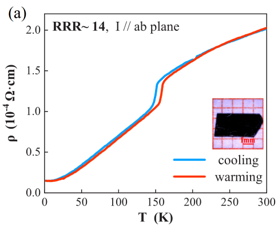
\includegraphics[width=\textwidth]{tate2/resistivity.png}
		\caption{}
	\end{subfigure}
	\caption{(a) 1T' RT phase of \ce{TaTe2} forming ribbons. (b) 1T" LT phase of \ce{TaTe2}, \ce{Ta} atoms move together forming heptameres. (c) Resistivity of \ce{TaTe2} as a function of temperature with an overall reduction in resistivity while cooling. A phase transition occurs at \qty{170}{\kelvin}, which is accompanied by a further steplike reduction in resistivity. (a) and (b) adapted from \cite{lin_evidence_2022}, (c) from \cite{hu_optical_2022}.}
	\label{fig:tate_structure}
\end{figure}

As previously mentioned, \ce{TaS2} and \ce{TaSe2} are considered prototypical CDW compounds \cite{bozin_crystallization_2023, shen_precursor_2023}, exhibiting a Peierls-like instability, characterized by a PLD, the opening of an electronic gap, and a Kohn anomaly.
Although \ce{TaTe2} shares these characteristics, its phase transition is even more elusive.
This lack of understanding stems from the electronic response to the phase transition, especially in comparison to its \ce{TaX2} sister compounds.
Typically, as seen in \ce{TaS2} and \ce{TaSe2}, cooling the sample through the CDW transition leads to an increase in resistivity due to the reduced density of states (DOS) near the Fermi level $E_F$.
Similarly, the reduction in DOS, and thus the loss of electrons carrying magnetic moments, should result in a drop in magnetic susceptibility while cooling through $T_s$.
In contrast, \ce{TaTe2}, which exhibits semimetallic behavior at room temperature, shows a decrease in resistivity and an increase in magnetic susceptibility, despite the presence of small gaps in the band structure \cite{sorgel_new_2006,hu_optical_2022,lin_evidence_2022}.
For this reason, the compound has been labeled a "strange" CDW material \cite{lin_evidence_2022}.

The end of section \ref{sec:cdw} already discussed the challenges posed by higher dimensionality and stronger interactions.
While both \ce{TaS2} and \ce{TaSe2} are often considered Peierls-like, the situation is more complex than in the original 1D metal proposed by Peierls.
In this context, the local-bonding picture becomes more significant, and the role of the Fermi surface is reduced.
The local-bonding picture can be understood as an analogy to molecular chemistry.
In TMDs, an electron deficiency leads to charge transfer from the dichalcogenide to the transition metal, resulting in shortened bonds and clustering.
The charge transfer from \ce{Te} to \ce{Ta} allows for the formation of local multi-center bonds, forming the double zigzag patterns, which may be a driving force behind the PLD formation in \ce{TaTe2} \cite{pouget_structural_2024, whangbo_analogies_1992, canadell_importance_1992, albright_thomas_a_orbital_2013}.

In the following sections, I will focus on the electronic band structure of \ce{TaTe2} and further explore the formation of its CDW phase at low temperatures, supported by trARPES data.
The local bonding picture discussed in this section will be crucial for interpreting the low-temperature phase, as well as for understanding the formation of a photo-induced metastable state.

\section{Bandstructure and Fermiology}

The electronic structure of \ce{TaTe2} is primarily governed by local molecular bonding between \ce{Ta}-\ce{Ta} dimers, with ARPES measurements revealing a complex set of bands in the room-temperature (RT) phase.
The valence states that control the electronic properties of this compound consist of a mixture of \ce{Ta} 5d and \ce{Te} 5p orbitals \cite{mitsuishi_unveiling_2024}.

The Fermi surface of \ce{TaTe2} displays a more pronounced quasi-1D character compared to other 2D materials, even when compared to its isostructural counterparts \ce{TaSe2} and \ce{TaS2} \cite{lin_evidence_2022}.
This quasi-1D nature is observed as two-fold symmetric wavy contours around \qty{0.5}{\angstrom^{-1}} along the $\Gamma$-M$_1$ direction, forming an outer Fermi surface.
Within these wavy contours lies a second, inner Fermi surface that forms multiple pockets (see Fig. \ref{fig:TaTe_FS} (b)).

\begin{figure}[t!]
	\centering
	\begin{subfigure}[b]{0.49\textwidth}
		\includegraphics[width=\textwidth]{tate2/TaTe2_BZ_sketch_full.pdf}
		\caption{}
	\end{subfigure}
	\hfill
	\begin{subfigure}[b]{0.49\textwidth}
		\includegraphics[width=\textwidth]{tate2/TaTe2_contours.png}
		\caption{}
	\end{subfigure}
	\\
	\begin{subfigure}[b]{0.49\textwidth}
		\includegraphics[width=\textwidth]{tate2/TaTe2_FS_RT.pdf}
		\caption{}
	\end{subfigure}
	\hfill
	\begin{subfigure}[b]{0.49\textwidth}
		\includegraphics[width=\textwidth]{tate2/TaTe2_FS_LT.pdf}
		\caption{}
	\end{subfigure}
	\caption{(a) The measured Fermi surface of the LT phase is overlapped with the 1. BZ of the virtual monoclinic (1 x 1) 1T phase (black), extended BZs of the distorted HT (3 x 1) 1T' phase (orange) and extended BZs of the further distorted LT (3 x 3) 1 T'' phase (red). (b) LT Fermi surface shown together with the contours of the inner and outer Fermi surface sheet for which nesting conditions can be fulfilled (c) RT Fermi surface overlapped with the HT and LT Brillouin zones. The relevant high symmetry points are marked. (d) Same Fermi surface as (c) but measured in the LT phase at \qty{77}{\kelvin}.}
	\label{fig:TaTe_FS}
\end{figure}

When comparing the RT and LT Fermi surfaces, only minor differences are observed.
The overall topology, with the wavy outer contours and the inner Fermi surface sheet with multiple pockets, remains largely conserved.
A notable distinction is the slight variation in the size of the pockets within the inner sheet, as well as more pronounced features in the second Brillouin zone (BZ) of the LT Fermi surface.
The pocket size difference results from a small shift in the chemical potential upon cooling through the phase transition, a change that has also been observed by N. Mitsuishi et al. \cite{mitsuishi_unveiling_2024}.

While the changes in Fermi surface topology are small, the effects of the phase transition become more apparent when examining the bandmaps.
A series of bandmaps taken parallel to the K$_2$-$\Gamma$-K$_2$ direction from the $\Gamma$-point to the second BZ boundary is compared for both room and low temperatures.

\begin{figure}[t!]
	\centering
	\includegraphics[width=0.9\textwidth]{tate2/TaTe2_RT_cuts.pdf}
	\caption{Series of cuts parallel to K$_1$-$\Gamma$-K$_1$, from $\Gamma$ to the BZ border. The location of the cuts in respect to the BZ is indicated in the FS of Fig. \ref{fig:TaTe_FS}. All cuts have been taken at RT, using the Helium $\alpha1$ line of a Helium lamp.}
	\label{fig:TaTe_RT_cuts}
\end{figure}

At RT, the bandmaps reveal a multitude of bands, with several crossing the Fermi level in each cut.
These Fermi crossings reveal the two Fermi sheets: the crossing at the edge of the band determines the wavy contours of the outer quasi-1D Fermi surface, while the crossing closer to the center of the band structure corresponds to the inner Fermi sheet.
Upon cooling through the phase transition, the bands undergo a complex reordering.
The broad bands observed in the RT phase split into multiple individual bands, and additional backfolded bands appear.
Looking at the FS crossing of the inner sheet, the aforementioned size difference of the Fermi pockets becomes clearer.
Comparing the cuts of the RT phase to the equivalent LT cuts, it is possible to identify a small shift in the chemical potential $\mu$, which has also been reported by \cite{mitsuishi_unveiling_2024}.
Another distinguishing feature between the RT and LT phases is the flattening of bands near $E_F$, at energies above \qty{-0.6}{\electronvolt}.

\begin{figure}[h]
	\centering
	\includegraphics[width=0.9\textwidth]{tate2/TaTe2_LT_cuts.pdf}
	\caption{Series of cuts parallel to K$_2$-$\Gamma$-K$_2$, from $\Gamma$ to the BZ border. The cuts are the equivalent band maps to the RT one in Fig. \ref{fig:TaTe_RT_cuts}. All cuts have been taken at LT $\simeq$\qty{77}{\kelvin}, using the Helium $\alpha1$ line of a Helium lamp.}
	\label{fig:TaTe_LT_cuts}
\end{figure}

The flattening of the bands may result from the established charge order in the LT phase, which typically leads to gap formation and backfolded bands due to the PLD.
To further understand the CDW and gap formation, we need to revisit the quasi-1D character of the FS.
Fermi surface nesting occurs when different regions of the Fermi surface can be connected by a reciprocal lattice vector, effectively translating the surfaces onto each other, as discussed in section \ref{sec:cdw}.
FSN can lead to charge instabilities near the FS and can play a significant role in CDW formation.
The wavy contours of the outer Fermi surface sheet (see Fig. \ref{fig:TaTe_FS}) can be translated onto each other, suggesting the presence of a FSN effect.
The distance between two points connected by this vector is approximately \qty{0.92}{\angstrom^{-1}}, which is comparable to the \qty{0.85}{\angstrom^{-1}} reported by Y. Lin et al. \cite{lin_evidence_2022}.
A possible second FSN vector is observed for the inner FS sheet, with a vector length of \qty{0.24}{\angstrom^{-1}}.
However, neither of these FSN vector lengths matches the periodicity of the PLD, which is $\simeq\qty{0.67}{\angstrom^{-1}}$.

Sections \ref{sec:cdw} and \ref{sec:cdw_tate2} discussed the complications introduced by higher dimensionality and stronger couplings, both of which are evident here.
Despite the presence of multiple possibly nested pockets, no matching lattice superstructure is observed.
Even in materials with quasi-1D Fermi surfaces, the influence of FSN is greatly diminished, as evidenced by the mismatch in vector amplitudes.
While FSN may contribute to the formation of the CDW by affecting the electron-hole susceptibility, it is not the sole or primary factor driving the formation of the LT phase.

As a result of CDW formation, small gaps can be observed across the Brillouin zone, most prominently near the $\Gamma$-point \cite{lin_evidence_2022}.
Figure \ref{fig:TaTe_minigaps} shows a cut near $\Gamma$, with a dashed box highlighting the region where minigaps form.
A zoomed-in view of this area better illustrates the small gaps near \qty{0.4}{\angstrom^{-1}} at the edge of the band map.
This band also connects to the wavy contours that meet the FSN condition, suggesting that an interplay between FSN and gap formation may still be relevant.

\begin{figure}[h!]
	\centering
	\includegraphics[width=0.7\textwidth]{tate2/TaTe2_CDW_minigaps.pdf}
	\caption{Left: Band map parallel to the K$_2$-$\Gamma$-K$_2$ direction close to the $\Gamma$-point. The dashed rectangle marks the region of which a zoom is provided. Right: Zoom of dashed rectangle region. The band map shows a faint signature of the observed minigaps \cite{lin_evidence_2022}.}
	\label{fig:TaTe_minigaps}
\end{figure}

\section{Ultrafast charge dynamics and CDW quench}
\label{sec:tate_dynamics}

Investigating the evolution of the electronic band structure following pump excitation provides valuable insight into the relaxation dynamics of not only isolated electronic states but also the collective response of the material out of equilibrium.
This is particularly beneficial for complex materials where multiple many-body effects may interact, influencing each other.
While static techniques capture the overall equilibrium state, time-resolved techniques help establish a hierarchy between the various phenomena, allowing for discrimination between different contributions.
In this context, performing pump-probe experiments at both room temperature and low temperature enables the exploration of differences between the two structural phases.
Throughout this chapter, the excitation is generated by an ultrashort laser pulse of \qty{1.6}{\electronvolt}.
I will begin by analyzing measurements in the low temperature phase at \qty{77}{\kelvin}, followed by a comparison to RT data to highlight the changes induced by the phase transition.

The LT cuts presented in this section are measured along the K$_2$-$\Gamma$-K$_2$ direction at three points in the LT FBZ ($\Gamma$, M$_1$ and near $\Gamma$).
Focusing on the cut close to $\Gamma$, we observe complex band dynamics that vary significantly across different regions of the band structure.
Figure \ref{fig:TaTe_bandmap_dyn_betw} shows this band map \qty{50}{\femto\second} after excitation, with difference maps at three selected time steps (\qtylist{50; 500; 4000}{\femto\second}) highlighting the pump-induced changes.

At \qty{50}{\femto\second}, a rapid depopulation of occupied bands is evident, with the difference contours closely following the equilibrium band structure.
Similarly, a fast population of unoccupied states is observed.
The close alignment of the contours with the unexcited band structure suggests that the signal corresponds to a change in population rather than a shift in the bands.
This is followed by an initial decay of the excitation, however, by \qty{500}{\femto\second}, a sudden increase in spectral weight is seen in the occupied states.
This trend change can be explained by a quench of the charge order, which will be discussed in more detail later in this section.
Notably, the region of intensity increase corresponds to where CDW minigaps form.
At \qty{4}{\pico\second}, most of the excited population has decayed, although some residual population remains, and the band structure is significantly altered compared to the equilibrium state.

\begin{figure}[t!]
	\centering
	\includegraphics[width=\textwidth]{tate2/bandmap_dyn_markers_betw.png}
	\caption{Left: Band map close to $\Gamma$ oriented along K$_2$-$\Gamma$-K$_2$ direction at a time delay of \qty{50}{\femto\second} after pump excitation. The other plots show difference maps at different time delays (\qtylist{50;500;4000}{\femto\second}). Rectangles show the regions for which dedicated delay traces are displayed in \ref{fig:TaTe_dyn_betw}. The difference map show characteristic features for each time steps. At \qty{50}{\femto\second} fast de-/population due to the pump excitation occurs. After \qty{500}{\femto\second} a population of a region below $E_F$ appears, corresponding to the closure of the CDW gap. After \qty{4}{\pico\second} the difference map shows regions where a change of the band structure and population above $E_F$ persists. Measurement was done at \qty{77}{\kelvin}.}
	\label{fig:TaTe_bandmap_dyn_betw}
\end{figure}

For more detailed insight into the relaxation dynamics, specific delay traces are examined (see Fig. \ref{fig:TaTe_dyn_betw}).
These traces, marked with squares in Fig. \ref{fig:TaTe_bandmap_dyn_betw}, are colored black for unoccupied regions, white for occupied states, and green for regions with significant spectral weight after \qty{4}{\pico\second}.
In the unoccupied regions (black squares, see Fig. \ref{fig:TaTe_dyn_betw} (a)-(c)), a sharp population occurs within the duration of the pump pulse, followed by a fast decay that becomes increasingly slower near $E_F$.
By \qty{4}{\pico\second}, the population has largely decayed.
Similarly, the depopulation of the occupied states in Fig. \ref{fig:TaTe_dyn_betw} (d) occurs within the pump pulse duration and recovers on the same timescale.

Unexpectedly, the dynamics in the region below $E_F$ (see Fig. \ref{fig:TaTe_dyn_betw} (e)) show an increase in population, rather than the typical reduction expected after pump excitation.
This unusual behavior is due to the small gaps formed by the CDW, which result in a loss of density of states (DOS) at equilibrium compared to the normal state.
If this charge order is broken a gap closure is expected to be observed and, in a first approximation excluding other band modification, a re-establishment of the RT DOS.
This behavior is observed in Fig. \ref{fig:TaTe_dyn_betw} (e), which coincides with the region of CDW gaps reported by \cite{lin_evidence_2022}.
Fitting a single exponential decay model to this trace yields a time zero of $t_0=\qty{388}{\femto\second}$, indicating a delay of about \qty{320}{\femto\second} compared to all other traces in Fig. \ref{fig:TaTe_dyn_betw}

\begin{figure}[t]
	\centering
	\begin{subfigure}[b]{0.33\textwidth}
		\includegraphics[width=\textwidth]{tate2/Unocc_dyn_1_fit_betw.pdf}
		\caption{}
	\end{subfigure}
	\hfill
	\begin{subfigure}[b]{0.33\textwidth}
		\includegraphics[width=\textwidth]{tate2/Unocc_dyn_2_fit_betw.pdf}
		\caption{}
	\end{subfigure}
	\hfill
	\begin{subfigure}[b]{0.33\textwidth}
		\includegraphics[width=\textwidth]{tate2/Unocc_dyn_3_fit_betw.pdf}
		\caption{}
	\end{subfigure}
	\\
	\begin{subfigure}[b]{0.33\textwidth}
		\includegraphics[width=\textwidth]{tate2/Occ_dyn_fit_betw.pdf}
		\caption{}
	\end{subfigure}
	\hfill
	\begin{subfigure}[b]{0.33\textwidth}
		\includegraphics[width=\textwidth]{tate2/CDW_quench_fit_betw.pdf}
		\caption{}
	\end{subfigure}
	\hfill
	\begin{subfigure}[b]{0.33\textwidth}
		\includegraphics[width=\textwidth]{tate2/Meta_dyn_fit_betw.pdf}
		\caption{}
	\end{subfigure}
	\caption{Delay traces of the regions marked in Fig. \ref{fig:TaTe_bandmap_dyn_betw} with the corresponding fit function of a single exponential decay model and resulting time constants $t_0$ and $\tau$. (a)-(c) Dynamics of unoccupied regions (black markers in Fig. \ref{fig:TaTe_bandmap_dyn_betw}) show fast population within pump pulse, followed with increasing relaxation time closer to $E_F$. (d)-(e) Dynamics of unoccupied regions (white markers in Fig. \ref{fig:TaTe_bandmap_dyn_betw}). (d) Fast depopulation within pump excitation. (e) Delayed response compared to $t_0$ and increased spectral weight. (f) Dynamics of region slightly above $E_F$ (green marker in Fig. \ref{fig:TaTe_bandmap_dyn_betw}) shows a instantaneous population within pump pulse, and persisting occupation beyond \qty{4}{\pico\second}.}
	\label{fig:TaTe_dyn_betw}
\end{figure}

This delayed response becomes particularly evident when the CDW quench dynamics are overlaid with the fast de-/population dynamics see Fig. \ref{fig:TaTe_CDW_comp}).
Many ultrafast studies have looked at the dynamics of the CDW and while the timescales typically differ, depending on the mechanism, a common observation is that the quench of the charge order starts together with the arrival of the pump pulse \cite{perfetti_time_2006, rohwer_collapse_2011, rettig_coherent_2014, shi_ultrafast_2019, maklar_nonequilibrium_2021, maklar_coherent_2022, huber_mapping_2022, huber_revealing_2022, maklar_coherent_2023, huber_ultrafast_2024}.
In contrast, here a quench on the timescale of few hundred \unit{\femto\second} is observed, which is typically associated with a Peierls type CDW, but the onset of the quench is delayed with respect to time zero $t_0$.
The delayed response rules out a solely electronic character and instead established the structural component as the dominant contribution for the CDW order in \ce{TaTe2}.
In other words, instead of the electromagnetic field of the pump pulse disrupting the charge order via buildup of free charges and subsequent ultrafast screening, the more likely scenario is a coherent response of the lattice, resulting in an excitation of phonon modes on ultrafast time scales, which couple to the charge order via the strong electron-phonon coupling of the system.

The slow response of the CDW to light appears as well when looking at the edge of the gapped region.
The corresponding dynamics, overlapped with the dynamics of the direct de-/population are shown in Fig. \ref{fig:TaTe_CDW_comp}.
In the trace an inital dip at $t_0$ can be seen, originating from the depopulation dynamics of the occupied band.
But after \qty{300}{\femto\second}, this depopulation is drowned out by the closing of the CDW gap.
It is quite remarkable that in adjacent energy-momentum coordinates vastly different dynamics can be observed.
A relaxation time of $\tau_{CDW}=\qty{500}{\femto\second}$ can be extracted by fitting a single exponential decay model, corresponding to the time duration to reestablish the charge order.

\begin{figure}[t!]
	\centering
	\begin{subfigure}[b]{0.33\textwidth}
		\includegraphics[width=\textwidth]{tate2/CDW_quench_multitrace_betw.pdf}
		\caption{}
	\end{subfigure}
	\begin{subfigure}[b]{0.33\textwidth}
		\includegraphics[width=\textwidth]{tate2/CDW_2_dyn_fit.pdf}
		\caption{}
	\end{subfigure}
	\caption{Left: Delay trace showing the dynamics of the CDW quench, overlapped with delay traces showing the direct de-/population of the occupied/unoccupied states, visualizing the delayed response of the CDW to the light excitation. Right: Dynamics of CDW quench combined with a fit of a single exponential decay model, resulting in a decay time of $\tau_{CDW}=\qty{460}{\femto\second}$ and an onset of the dynamic at $t=\qty{420}{\femto\second}$.}
	\label{fig:TaTe_CDW_comp}
\end{figure}

The residual spectral weight visible in the difference map at \qty{4}{\pico\second} (see Fig. \ref{fig:TaTe_bandmap_dyn_betw}) further supports the idea of a long lived state.
The corresponding delay trace (green square in Fig. \ref{fig:TaTe_dyn_betw} (f)) shows a fast population within the pump pulse duration, followed by an initial decay.
However, the population does not return to its initial state.
Instead, a sharp feature appears above $E_F$ in the bandmap of figure \ref{fig:TaTe_bandmap_dyn_betw}.
A more detailed analysis of this feature, including measurements on longer time scales, will be done in section \ref{sec:meta}.
Comparing all traces reveals a common feature: strong coherent oscillations of the intensity, which will be discussed in detail in the next section \ref{sec:phonon_osc}.

\begin{figure}[t!]
	\centering
	\begin{subfigure}[b]{\textwidth}
		\includegraphics[width=\textwidth]{tate2/bandmap_dyn_markers_gamma.png}
		\caption{}
	\end{subfigure}
	\\
	\centering
	\begin{subfigure}[b]{\textwidth}
		\includegraphics[width=\textwidth]{tate2/bandmap_dyn_markers_bzb.png}
		\caption{}
	\end{subfigure}
	\\
	\begin{subfigure}[b]{0.33\textwidth}
		\includegraphics[width=\textwidth]{tate2/CDW_quench_multitrace_gamma.pdf}
		\caption{}
	\end{subfigure}
	\begin{subfigure}[b]{0.33\textwidth}
		\includegraphics[width=\textwidth]{tate2/CDW_quench_multitrace_bzb.pdf}
		\caption{}
	\end{subfigure}
	\caption{Figure similar to Fig. \ref{fig:TaTe_bandmap_dyn_betw} for different cuts. (a) Cut through $\Gamma$. (b) Cut through M$_1$. Both cuts are along the K$_2$-$\Gamma$-K$_2$ direction. (c) \& (d) show trace of the CDW quench plotted together with the direct excitation of the unoccupied states.}
	\label{fig:TaTe_bandmap_dyn_bzb}
\end{figure}

The described dynamics are not confined to regions near $\Gamma$ but can also be observed at the $\Gamma$-point directly and at the edge of the FBZ at M$_1$ (see Fig. \ref{fig:TaTe_FS} (d)).
Figure \ref{fig:TaTe_bandmap_dyn_bzb} shows the excited band map at M$_1$ at $t_0$, along with difference maps at specific time delays.
The same instantaneous de-/population of the occupied/unoccupied bands and a by several hundred \unit{\femto\second} delayed CDW gap quench are visible (see Fig. \ref{fig:TaTe_bandmap_dyn_bzb} (c)-(d)).
The only notable difference is the absence of residual spectral weight at M$_1$, likely due to the lower pump fluence used in these measurements.

Comparing the LT and RT phases reveals significant differences in the band structure dynamics for an equivalent cut close to $\Gamma$ (see Fig. \ref{fig:TaTe_bandmap_dyn_betw_rt}.
First a direct population of the occupied states can be observed within the pump pulse duration.
But, unlike the LT case, the population seems to be disproportionately located in the region just above $E_F$, whereas the unoccupied states at higher energies appear to be less populated.
While the LT phase was additionally characterized by strong changes to the band structure after the first few hundred \unit{\femto\second}, no changes occur in the RT phase.
Instead, the population of the unoccupied bands, as well as the depopulation of the occupied parts simply decays.
After \qty{3}{\pico\second} some spectral weight still remains close to $E_F$, but no discrete spectral feature can be observed.
The full time dynamic for selected regions, which are marked by squares in Fig. \ref{fig:TaTe_bandmap_dyn_betw_rt}, can be seen in Fig. \ref{fig:TaTe_dyn_betw_rt}.
Those traces show similar relaxation times as the LT ones.

\begin{figure}[t!]
	\centering
	\includegraphics[width=\textwidth]{tate2/diffmap_dyn_markers_betw_rt.png}
	\caption{Left: Band map close to $\Gamma$ oriented along K$_2$-$\Gamma$-K$_2$ direction \qty{50}{\femto\second} after pulse excitation. The other plots show difference maps at different time delays (\qtylist{50;400;3000}{\femto\second}). Rectangles show the regions for which dedicated delay traces are displayed in \ref{fig:TaTe_dyn_betw_RT}. The difference map shows the ultrafast de-/population after pump excitation, followed by a decay and a small diffuse residual spectral weight after \qty{3}{\pico\second}. No changes to the band structure apart from de-/population dynamics can be observed.}
	\label{fig:TaTe_bandmap_dyn_betw_rt}
\end{figure}

\begin{figure}[b!]
	\centering
	\begin{subfigure}[b]{0.24\textwidth}
		\includegraphics[width=\textwidth]{tate2/Unocc_dyn_1_fit_betw_rt.pdf}
		\caption{}
	\end{subfigure}
	\begin{subfigure}[b]{0.24\textwidth}
		\includegraphics[width=\textwidth]{tate2/Unocc_dyn_2_fit_betw_rt.pdf}
		\caption{}
	\end{subfigure}
	\begin{subfigure}[b]{0.24\textwidth}
		\includegraphics[width=\textwidth]{tate2/Unocc_dyn_3_fit_betw_rt.pdf}
		\caption{}
	\end{subfigure}
	\begin{subfigure}[b]{0.24\textwidth}
		\includegraphics[width=\textwidth]{tate2/Occ_dyn_fit_betw_rt.pdf}
		\caption{}
	\end{subfigure}
	\caption{
		Delay traces of the regions marked in Fig. \ref{fig:TaTe_bandmap_dyn_betw_rt} with the corresponding fit function of a single exponential decay model and resulting time constants $t_0$ and $\tau$. (a)-(c) Dynamics of unoccupied regions (black markers in Fig. \ref{fig:TaTe_bandmap_dyn_betw_rt}) show fast population within pump pulse, followed with increasing relaxation time closer to $E_F$. (d) Dynamic of unoccupied regions (white markers in Fig. \ref{fig:TaTe_bandmap_dyn_betw_rt}) shows fast depopulation within pump excitation and small residual spectral weight after \qty{3}{\pico\second}.}
	\label{fig:TaTe_dyn_betw_rt}
\end{figure}

Two key differences emerge from the RT data:
First, the absence of a spectral feature at \qty{500}{\femto\second}(see Fig. \ref{fig:TaTe_dyn_betw_rt}), as well as an absence of band reordering.
Second while some residual spectral weight remains after \qty{3}{\pico\second}, it is diffuse and lacks the sharp features seen in the LT phase.

These results suggest that the high temperature phase is more resistant to photoexcitation.
For example, no evidence of a transition to a hypothetical undistorted structure could be identified, consistent with previous ultrafast structural studies \cite{domrose_femtosecond_2024}.
This absence of distinct spectral changes at HT is also remarkable, due to the fact that stripe-like charge ordering exists in the HT phase.
In contrast, the LT phase shows that the charge order can be melted with ultrafast light pulses, leading to the increased population below $E_F$.
Indeed, ultrafast structural studies \cite{domrose_femtosecond_2024, siddiqui_ultrafast_2021} have reported on a partial melting of the PLD.
The complex reformation of bands might be as well a direct consequence of this.
The delayed CDW quench points to a strong structural component of the CDW/PLD.
The residual spectral weight above $E_F$ in the LT phase further indicates the existence of a metastable state.

As shown throughout this section, the time dynamics vary significantly across different regions in energy and momentum space.
The next section will focus on momentum- and energy-dependent dynamics in more detail.
Additionally, the residual spectral weight will be discussed in terms of a metastable state in section \ref{sec:meta}.

\section{Energy and momentum resolved electron-phonon coupling}
\label{sec:phonon_osc}

In the previous section, we examined the dynamics at both low and room temperatures, revealing strong momentum- and energy-dependent oscillations in the intensity of each trace.
These oscillations are the focus of this section.

Coherent oscillations in delay traces of trARPES measurements are typically indicative of phonon interactions.
ARPES measures only the single-particle spectral function, so quasiparticles like phonons themselves cannot be directly observed.
Instead, information about phonons is imprinted on the measured photoelectrons through electron-phonon coupling.
When this coupling is sufficiently strong, it is possible to observe oscillations in the time traces of a trARPES experiment.
Several mechanisms can lead to coherent phonon excitation, including various Raman scattering processes, as well as infrared absorption, and displacive excitation of coherent phonons (DECP) \cite{zeiger_theory_1992, kuznetsov_theory_1994, giret_entropy_2011, juraschek_sum-frequency_2018, lakehal_microscopic_2019, caruso_quantum_2023, emeis_coherent_2024}.
In semi-metals, DECP is usually the dominant excitation pathway.
In this process, photons from the pump pulse are absorbed, creating a quasi-adiabatic displacement of the potential energy surface.
The lattice then responds by oscillating coherently around the minimum of the displaced energy surface, a motion that dephases over time as the phonon damps out \cite{zeiger_theory_1992, kuznetsov_theory_1994, bothschafter_ultrafast_2013, emeis_coherent_2024}.

Ditellurides, especially \ce{TaTe2}, exhibit exceptionally high electron-phonon coupling.
This strong coupling allows for the observation of oscillations not just over large, integrated regions of the band structure, but also at each individual momentum and energy coordinate.
This characteristic provides an opportunity to perform a band mapping of the electron-phonon coupling over large regions of energy-momentum space.
By performing a Fourier analysis on the delay traces, the frequency of the oscillations can be extracted and assigned to specific vibrational modes.
To my knowledge, this is the first time such an energy- and momentum-resolved Fourier analysis of electron-phonon coupling has been performed in ARPES using high harmonic generation as a probe.

\begin{figure}[b!]
	\centering
	\includegraphics[width=\textwidth]{tate2/tate_fit_procedure.pdf}
	\caption{Left: Band map close to $\Gamma$ oriented along K$_2$-$\Gamma$-K$_2$ direction \qty{50}{\femto\second} after pulse excitation. The other plots show difference maps at different time delays (\qtylist{50;400;3000}{\femto\second}). Rectangles show the regions for which dedicated delay traces are displayed in \ref{fig:TaTe_dyn_betw_RT}. The difference map shows the ultrafast de-/population after pump excitation, followed by a decay and a small diffuse residual spectral weight after \qty{3}{\pico\second}. No changes to the band structure apart from de-/population dynamics can be observed.}
	\label{fig:TaTe_fit_procedure}
\end{figure}

In this procedure, the raw data is first binned over four pixels in both the momentum and energy coordinates to slightly increase the signal-to-noise ratio and reduce the computational load, with minimal sacrifice to the fidelity of the bandmaps.
An analytic function, reproducing the fast population or depopulation after pump excitation and the subsequent decay, is fitted to each $E(k)$-coordinate.
The analytic function is defined as
\begin{equation}
	A + \frac{1}{2} \left( B \cdot \exp\left(\frac{t_0-t}{\tau} + \frac{\sigma}{\tau}\right) \right) \cdot \left( 1 + \text{erf}\left(\frac{t-t_0-\frac{2\sigma}{\tau}}{\sigma\sqrt{2}}\right) \right) + C \frac{1}{2} \left( 1 + \text{erf}\left(\frac{t-t_0}{\sigma\sqrt{2}}\right) \right)
	\label{eq:decay_model}
\end{equation}
with time zero $t_0$, decay time $\tau$ and a broadening $\sigma$.
The error function $\text{erf}(z)$ is given by
\begin{equation}
	\text{erf}(z) = \frac{2}{\sqrt{\pi}} \int_{t=0}^{z} \exp(-t^2)
\end{equation}
After subtracting this exponential decay from the raw data, the residual trace contains only the oscillatory components.
A fast Fourier transform (FFT) from the scipy Python package \cite{noauthor_rfft_nodate} is then applied to these residual traces, revealing the frequencies of the oscillatory components.
In this case, the dataset consists of 60 delay steps, and the FFT function is defined over 200 points, applying a zero-padding of 140 points.
The FFT transforms the original 3D data cube from $I(E,k,t)$ to $I(E,k,f)$, with frequency $f$ being the Fourier-transformed time axis.
Fig. \ref{fig:TaTe_fit_procedure} shows the steps from a delay trace to the FFT trace that can be associated with a particular phonon mode.

Performing this analysis for a cut near $\Gamma$ reveals three distinct vibrational modes in the LT phase (see Fig. \ref{fig:TaTe_FFT_betw} (c)) at \qtylist{0.4; 1.45; 2.3}{\tera\hertz}.
Two modes (\qtylist{1.45; 2.3}{\tera\hertz}) have been previously observed using Raman spectroscopy and ultrafast transient reflectivity \cite{luo_subtle_2021, hu_optical_2022}, while the \qty{0.4}{\tera\hertz} mode has not been reported before.
Figure \ref{fig:TaTe_FFT_betw} (b)) shows the corresponding bandmaps at \qty{50}{\femto\second} after pump excitation for these frequencies.
It is important to note that these maps do not directly represent the phonon modes but rather the effect of the phonons on the band structure mediated by electron-phonon coupling.
The strong coupling allows for a high-resolution mapping of this coupling across both energy and momentum, revealing band-specific interactions.

The coupling maps closely follow the spectral weight distribution of the band structure.
Additionally, each phonon mode is seen to couple to specific regions of the band structure.
Notably, the features associated with the \qty{0.4}{\tera\hertz} mode correspond to the regions where CDW gaps were observed to close in the previous section.
Integrating over the entire energy and momentum space yields the trace shown in Fig. \ref{fig:TaTe_FFT_betw} (c), highlighting the presence of the three phonon modes.

\begin{figure}[b!]
	\centering
	\begin{subfigure}[b]{0.24\textwidth}
		\includegraphics[width=\textwidth]{tate2/tate_FFT_ref_betw.pdf}
		\caption{}
	\end{subfigure}
	\begin{subfigure}[b]{0.72\textwidth}
		\includegraphics[width=\textwidth]{tate2/tate_FFT_betw.pdf}
		\caption{}
	\end{subfigure}
	\\
	\begin{subfigure}[b]{0.33\textwidth}
		\includegraphics[width=\textwidth]{tate2/tate_FFT_summed.pdf}
		\caption{}
	\end{subfigure}
	\caption{Figure similar to Fig. \ref{fig:TaTe_bandmap_dyn_betw} for different cuts. (a) Cut through $\Gamma$. (b) Cut through M$_1$. Both cuts are along the K$_2$-$\Gamma$-K$_2$ direction. (c) \& (d) show trace of the CDW quench plotted together with the direct excitation of the unoccupied states.}
	\label{fig:TaTe_FFT_betw}
\end{figure}

In Fig. \ref{fig:TaTe_FFT_traces_betw} some exemplary time traces are shown in (a) with their corresponding FFT traces in (b).
These traces illustrate the differences between the phonon modes and provide further insight into their behavior.
The \qtylist{1.45; 2.3}{\tera\hertz} phonon modes oscillate around the exponential decay, while the \qty{0.4}{\tera\hertz} mode strongly modulates the intensity, almost causing a re-population after the decay has already set in.
Furthermore, the oscillations due to electron-phonon coupling start immediately after the IR pump pulse, while the closure of the CDW gap is delayed by several hundred femtoseconds.
This supports the idea that the CDW is not disrupted immediately by the light pulse, but through the interaction with the phonons, with the CDW gap closing around \qty{350}{\femto\second}.
Similar results are observed for the other cuts at $\Gamma$ and M$_1$, analyzed previously.
Both cuts show the three phonon modes listed above and show them couple to different bands in the band structure.

\begin{figure}[t!]
	\centering
	\begin{subfigure}[b]{\textwidth}
		\includegraphics[width=\textwidth]{tate2/Osc_time_traces_betw.pdf}
		\caption{}
	\end{subfigure}
	\\
	\begin{subfigure}[b]{\textwidth}
		\includegraphics[width=\textwidth]{tate2/Osc_freq_traces_betw.pdf}
		\caption{}
	\end{subfigure}
	\caption{Figure similar to Fig. \ref{fig:TaTe_bandmap_dyn_betw} for different cuts. (a) Cut through $\Gamma$. (b) Cut through M$_1$. Both cuts are along the K$_2$-$\Gamma$-K$_2$ direction. (c) \& (d) show trace of the CDW quench plotted together with the direct excitation of the unoccupied states.}
	\label{fig:TaTe_FFT_traces_betw}
\end{figure}

\begin{figure}[b!]
	\centering
	\includegraphics[width=\textwidth]{tate2/cosine_fit.png}
	\caption{Figure similar to Fig. \ref{fig:TaTe_bandmap_dyn_betw} for different cuts. (a) Cut through $\Gamma$. (b) Cut through M$_1$. Both cuts are along the K$_2$-$\Gamma$-K$_2$ direction. (c) \& (d) show trace of the CDW quench plotted together with the direct excitation of the unoccupied states.}
	\label{fig:TaTe_cosine}
\end{figure}

Since the \qty{0.4}{\tera\hertz} mode lies at the lower end of the Fourier trace, it is essential to exclude the possibility that it is an artifact.
To verify this, a cosine curve is fitted along with the decay model from Eq. \ref{eq:decay_model} and the frequency of the cosine function is extracted. 
This fit function is given by
\begin{equation}
	f_\text{decay}(t) + f_\text{step}(t, t_0) * A * \cos(2\pi t+\phi) + C
\end{equation}
with $f_\text{decay}$ being the decay model of equation \ref{eq:decay_model}, an offset phase $\phi$ and a step function $f_\text{step}$.
The step function is necessary because the oscillation only occur at or after time zero $t_0$.
Repeating this fit procedure for traces that show the \qty{0.4}{\tera\hertz} mode in Fig. \ref{fig:TaTe_FFT_betw}, confirms that the delay traces can be fitted by a cosine function with a frequency of \qty{0.4}{\tera\hertz}.
An example of this fit procedure can be seen in Fig. \ref{fig:TaTe_cosine}.

One of the central questions regarding \ce{TaTe2} is the nature of its CDW.
The previous section presented evidence of the CDW's strong structural character, revealed through its delayed response to light excitation.
Now, I want to address the question of a possible amplitude mode.
A defining feature of an amplitude mode is that it vanishes when crossing from the CDW phase into the HT phase.
To investigate this, it is again necessary to look at the RT data and see how the oscillations change in the normal state.

\begin{figure}[b!]
	\centering
	\begin{subfigure}[b]{0.33\textwidth}
		\includegraphics[width=\textwidth]{tate2/tate_FFT_ref_betw_rt.pdf}
		\caption{}
	\end{subfigure}
	\begin{subfigure}[b]{0.66\textwidth}
		\includegraphics[width=\textwidth]{tate2/tate_FFT_betw_rt.pdf}
		\caption{}
	\end{subfigure}
	\\
	\begin{subfigure}[b]{0.33\textwidth}
		\includegraphics[width=\textwidth]{tate2/tate_FFT_summed_rt.pdf}
		\caption{}
	\end{subfigure}
	\caption{Figure similar to Fig. \ref{fig:TaTe_bandmap_dyn_betw} for different cuts. (a) Cut through $\Gamma$. (b) Cut through M$_1$. Both cuts are along the K$_2$-$\Gamma$-K$_2$ direction. (c) \& (d) show trace of the CDW quench plotted together with the direct excitation of the unoccupied states.}
	\label{fig:TaTe_FFT_betw_rt}
\end{figure}

In the RT data, the absence of the \qty{0.4}{\tera\hertz} mode (see Fig. \ref{fig:TaTe_FFT_betw_rt} (c)) is immediately noticeable.
This absence is a strong indicator that this mode may be an amplitude mode.
Other evidence also supports this, including the fact that the \qty{0.4}{\tera\hertz} mode directly couples to regions where the CDW gaps form and that its oscillations strongly modulate the intensity in the traces.
In addition to the disappearance of the amplitude mode, there are changes to the other two phonon modes.
Both modes exhibit a slight redshift and broadening in the RT phase.
Furthermore, the \qty{1.35}{\tera\hertz} mode now couples to a broader region of the band structure, while the \qty{2.2}{\tera\hertz} mode remains largely unchanged (see Fig. \ref{fig:TaTe_FFT_betw_rt} (b)).
The \qty{1.35}{\tera\hertz} mode now incorporates a broader region in the band structure at the edge of the band map, as well as the band in the center, which coupled to the \qty{0.4}{\tera\hertz} mode at LT.

These observations provide further insight into the structural phase transition and CDW formation in \ce{TaTe2}.
Two phonon modes persist in both the LT and HT phases, consistent with previous transient reflectivity and Raman spectroscopy studies \cite{hu_optical_2022, luo_subtle_2021}, although the \qty{1.45}{\tera\hertz} mode only appeared in the LT data of \cite{hu_optical_2022}.
The \qty{2.3}{\tera\hertz} mode appears largely unaffected by the phase transition, apart from a small redshift, and the band-resolved electron-phonon coupling remains the same, suggesting that this mode does not play a significant role in the transition.
In contrast, the \qty{1.45}{\tera\hertz} mode shows significant changes in band-specific coupling, particularly near $\Gamma$ and in regions of minigap formation.
At LT, the \qty{0.4}{\tera\hertz} mode emerges in these regions, coupling to bands affected by CDW gap formation.

A potential explanation for these observations lies in the local orbital character of the bands and the involvement of \ce{Ta} d-orbitals near $E_F$ \cite{mitsuishi_unveiling_2024}.
During the structural transition, the \ce{Ta} $d_{xy}$ orbital is strongly affected by the formation of heptamers, while the \ce{Te} atoms adjust to the new lattice distortion.
From a local bonding perspective, changes in bond length and overlap result in modifications to the effective electron count of the heptamers, compared to the fluctuating dimer state.
Therefore, the change in crystal structure has a profound impact on the band structure as well as the electron-phonon coupling.
These structural changes significantly impact both the band structure and electron-phonon coupling, enabling the formation of the LT CDW, mediated through a coupling between lattice and charges via the \qty{0.4}{\tera\hertz} phonon mode.

\section{Metastability}
\label{sec:meta}

Lastly I want to focus on the residual spectral weight, that was shown in the LT phase dynamics see \ref{fig:TaTe_bandmap_dyn_betw}.
Recently two groups have reported on a metastable state persisting into the \unit{\nano\second} regime, observed in pump probe electron diffraction measurements \cite{siddiqui_ultrafast_2021, domrose_femtosecond_2024}.
While these results can show the existence of a metastable state, the formation of this state remains elusive.
The diffraction studies can only provide insight on the structural dynamics of the material, but especially for compounds with such strong electron-phonon coupling it is imperative to also understand the electronic side of the out of equilibrium dynamics in order to disentangle the multiple different reordering and relaxation processes.
In the previous sections I already introduced the ultrafast electronic dynamics on shorter time scales up to \qty{4}{\pico\second}.
But for the discussion of the metastable state I will concentrate on the possible long term modifications of the electronic band structure and the different time scales leading up to the metastable state, by analyzing the longer time scales up to \qty{200}{\pico\second} after pump excitation.
For this, pump probe measurements of the valence states, as well as the Te 4d core states have been performed, both in the LT and HT phase.

\begin{figure}[b!]
	\centering
	\begin{subfigure}[b]{0.25\textwidth}
		\includegraphics[width=\textwidth]{images/tate2/meta_bandmap_marker}
		\caption{}
	\end{subfigure}
	\\
	\begin{subfigure}[b]{\textwidth}
		\includegraphics[width=\textwidth]{images/tate2/tate_lt_meta_steps}
		\caption{}
	\end{subfigure}
	\caption{(a) Bandmap of a cut close to $\Gamma$ along the K$_2$-$\Gamma$-K$_2$ direction similar to Fig. \ref{fig:TaTe_bandmap_dyn_betw} taken at $t_0$. Black markers show regions of the time traces shown in Fig. \ref{fig:metastableedge} (c)-(f). Region between two dashed lines corresponds to (a), region above higher dashed line to (b). (b) Difference maps showing the relative changes compared to before $t_0$ at selected time delays from $t_0$ to \qty{200}{\pico\second} after excitation. Measurement has been performed in the LT phase at approximately \qty{77}{\kelvin}.}
	\label{fig:tateltmetasteps}
\end{figure}

I will first focus on the dynamics of the band structure as a whole by looking at difference maps of a momentum cut close to BZ center.
The cut was taken in the LT phase at $\approx$\qty{77}{\kelvin} in the  K$_2$-$\Gamma$-K$_2$ direction, similar to Fig. \ref{fig:TaTe_bandmap_dyn_betw}.
In this measurement the range of delay steps was increased, measuring with a relatively fine step size of \qty{250}{\femto\second} from before $t_0$ to \qty{5}{\pico\second}, followed by progressively increasing step sizes up to \qty{200}{\pico\second} after pulse excitation.
The corresponding band map \qty{250}{\femto\second} after pulse excitation is shown in \ref{fig:tateltmetasteps} (a), together with the difference maps at selected time delays in Fig. \ref{fig:tateltmetasteps} (b).
In the first four difference maps between \qtyrange{250}{2000}{\femto\second} the same dynamics, which have been discussed in the previous section can be observed.
First an immediate population \& depopulation of the respective states occurs, which is followed by a delayed response of the charge order and a full quench of the CDW gaps $\approx$\qty{500}{\femto\second} after laser excitation.
The charger order recovers within \qty{1.5}{\pico\second} after the phonon mediated quench occurred.
During this recovery a reordering of the band structure sets in.
This transient reordering stabilizes after \qty{5}{\pico\second} and settles into band structure distinctly different from the equilibrium structure.
The new electronic structure is stable beyond \qty{200}{\pico\second} after excitation and fully recovers on \unit{\milli\second} timescales.

\begin{figure}[b!]
	\centering
	\begin{subfigure}[b]{0.33\textwidth}
		\includegraphics[width=\textwidth]{images/tate2/metastable_edge}
		\caption{}
	\end{subfigure}
	\begin{subfigure}[b]{0.33\textwidth}
		\includegraphics[width=\textwidth]{images/tate2/metastable_high}
		\caption{}
	\end{subfigure}
	\begin{subfigure}[b]{0.33\textwidth}
		\includegraphics[width=\textwidth]{images/tate2/metastable_occ}
		\caption{}
	\end{subfigure}
	\\
	\begin{subfigure}[b]{0.33\textwidth}
		\includegraphics[width=\textwidth]{images/tate2/metastable_state_ef}
		\caption{}
	\end{subfigure}
	\begin{subfigure}[b]{0.33\textwidth}
		\includegraphics[width=\textwidth]{images/tate2/metastable_left}
		\caption{}
	\end{subfigure}
	\begin{subfigure}[b]{0.33\textwidth}
		\includegraphics[width=\textwidth]{images/tate2/metastable_cdw}
		\caption{}
	\end{subfigure}
	\caption{Delay traces from \qtyrange{-1}{200}{\pico\second} for different regions close to $\Gamma$ as marked in Fig. \ref{fig:tateltmetasteps} (a) Inset shows a smaller time window (\qtyrange{-1}{10}{\pico\second}) with finer step size. Vertical dashed lines in the inset show the relaxation of the CDW and the coinciding band reordering at \qty{2}{\pico\second}. (a) Region close to the Fermi level, between the 2 dashed lines. (b) Region of unoccupied states at higher energies beyond (a). (c)-(f) Traces for regions marked with black squares. (c) Metastable depopulation of occupied state. (d) Metastable population of spectral feature above $E_F$, shows a delayed formation. (e) Fast depopulation of an occupied state, followed by a delayed reaction due to the band reordering. (f) Ultrafast depopulation of unoccupied state with CDW quench and subsequent band reordering. All traces taken at approximately \qty{77}{\kelvin}.}
	\label{fig:metastableedge}
\end{figure}

Following the time traces for selected features in the band structure provides a more detailed insight into the time evolution.
Selected traces are shown in Fig. \ref{fig:metastableedge}, with the corresponding regions of (c)-(f) marked by squares in Fig. \ref{fig:tateltmetasteps}.
Fig. \ref{fig:tateltmetasteps} (a) \& (b) correspond to the full range of momentum and for an energy $E_{kin}=E_F-E$ from \qtyrange{0}{0.15}{\electronvolt} or \qtyrange{0.15}{1.5}{\electronvolt} respectively (marked by the black dotted lines in Fig \ref{fig:tateltmetasteps} (a)).
Traces (a) \& (b) illustrate well the changes observed in the difference maps.
Above \qty{150}{\milli\electronvolt} a instantaneous population is observed, which has fully decayed after \qty{2}{\pico\second}, with no trace of any metastability.
Only in region between $E_F$ and \qty{150}{\milli\electronvolt} can a persistent occupation be observed.
Here after the initial excitation, the population decays and stabilizes after \qty{10}{\pico\second} and barely changes in intensity until \qty{200}{\pico\second} after pump excitation.
A similar behavior can be observed in the occupied states for trace (c) where, after the initial depopulation, the intensity is stable until after \qty{200}{\pico\second}.

Trace (d) provides a more detailed insight into the formation dynamics, by tracing the region in which the distinct spectral feature is formed above $E_F$ ($k_\parallel\approx$\qty{0.5}{\angstrom^{-1}}).
There, a first instantaneous population is again observed with a similar decay as in (b).
But instead of a full decay, a rise in intensity is observed at \qty{1}{\pico\second}, reaching a maximum at \qty{2}{\pico\second}, coinciding with the reformation of the CDW.
After reaching the maximum a small decay is observed until \qty{5}{\pico\second} at which the bands have settled into their persistent structure.
Similar behavior can for trace (e), where a depopulation is first observed, which then changes to a population above the base level between \qtyrange{1}{2}{\pico\second}, with a subsequent decay up to a delay of \qty{5}{\pico\second}, after which the intensity stabilizes.
Lastly trace (f) covers the region previously identified as the CDW minigap region.
Again, it is possible to see the immediate decay after pulse excitation, followed a stark overshoot in intensity due to the closing of the CDW gap at \qty{500}{\femto\second} (first dashed line in inset).
The overshoot decays and reaches close to the intensity value before $t_0$, after which the intensity rises again and settles at a slightly elevated level after \qty{10}{\pico\second}.

The time traces of the valence states confirm the discussion of the ultrafast dynamics from section \ref{sec:tate_dynamics}.
The excitation of \ce{TaTe2} is followed by a first ultrafast decay, after approximately \qty{450}{\femto\second} a quench of the CDW sets in.
Afterwards the charge order reforms on the timescale of \qty{2}{\pico\second}, mediated by the onset of the \qty{0.4}{\tera\hertz} phonon.
The reformation process is paired with a complex reordering of the band structure, which settles into a new quasi-equilibrium after \qty{5}{\pico\second} and is stable for more than \qty{200}{\pico\second}.

\begin{figure}[t!]
	\centering
	\begin{subfigure}[b]{0.33\textwidth}
		\includegraphics[width=\textwidth]{images/tate2/low_t}
		\caption{}
	\end{subfigure}
	\\
	\begin{subfigure}[b]{0.49\textwidth}
		\includegraphics[width=\textwidth]{images/tate2/low_energy_core_shift}
		\caption{}
	\end{subfigure}
	\hfill
	\begin{subfigure}[b]{0.49\textwidth}
		\includegraphics[width=\textwidth]{images/tate2/high_energy_core_shift}
		\caption{}
	\end{subfigure}
	\caption{(a) Bandmap showing the two \ce{Te} 4d levels. (b) Peak position of the upper 4d state from (a) is shown as a function of time after pump excitation for both RT and LT. Only the LT peak position shows a persistent shift to lower $E_B$.}
	\label{fig:tate_core}
\end{figure}

In addition to the valence states it is also possible to look at the evolution of the out of equilibrium dynamics of the core states by increasing the probe photon energy.
For this, a \qty{90}{\electronvolt} probe pulse was used to track the \ce{Te} 4d levels with a binding energy of \qty{41}{\electronvolt}.
A bandmap of these states is shown in Fig. \ref{fig:tate_core} (a).
The peak of both core levels is extracted from a double Gaussian fit as a function of time, both for RT and at \qty{77}{\kelvin}, in order to explore their evolution after pump excitation.
Fig. \ref{fig:tate_core} (b) (upper level) and (c) (lower level) show the peak position for up to \qty{50}{\pico\second} after pump excitation.
A sharp increase in binding energy can be seen for both the RT and the LT phase, corresponding to a shift of around \qty{40}{\milli\electronvolt}.
After this sudden shift a relaxation occurs within few \unit{\pico\second} before the band return to the equilibrium position after around \qty{5}{\pico\second} in the RT phase.
While in the LT phase a similar relaxation timescale can be observed, the core level does not relax back to the equilibrium energy position, but rather overshoots to a binding energy \qty{30}{\milli\electronvolt} below its equilibrium.
The overshoot is followed by a second relaxation, before the band settles at a binding energy $E_B=\qty{15}{\milli\electronvolt}$ below the original position, not relaxing back in the following \qty{45}{\pico\second}.


Apart from the existence of this metastable state and the obvious implication from a application/engineering perspective e.g. switches or opto-electronic devices \cite{bao_light-induced_2022, schaibley_valleytronics_2016,tokura_emergent_2017,konstantatos_current_2018,liu_semimetals_2020,du_engineering_2021}, the existence of the state might as well help us understand the fundamental physics of the equilibrium phase transition in \ce{TaTe2}.
Reports on the structure of \ce{TaTe2} have suggested that the ribbons in it's HT phase consist of fluctuating dimer bonds rather than stable trimers of \ce{Ta} atoms \cite{katayama_observation_2023}.
In addition, STM studies suggest that the HT (3 x 1)-symmetry coexists at LT with the (3 x 3) structure, with the two symmetries being in competition \cite{feng_charge_2016}.
From the structural perspective it therefore seems reasonable to suggest that, while the material settles into it's observed LT state when cooled adiabatically, these fluctuations and resulting competition enable the existence of local minima in the free energy landscape.

Perturbing the LT ground state of the material clearly does not only lead to an excitation of the electron bath, but instead launches many strongly coupled phonons, likely via DECP.
This perturbation of the lattice through vibrational modes destabilizes the charge order, which further has an impact on the out of equilibrium structure.
While a decay back to equilibrium at RT or in the HT phase should lead to a return to the equilibrium structure, it is clearly not the case when the decay is accelerated through the lower temperature, effectively freezing the structure and the electronic order.
A persistent change of the crystal structure, similar to persistent changes of the electronic structure, has been observed in previous ultrafast electron diffraction measurements \cite{siddiqui_ultrafast_2021, domrose_femtosecond_2024}, where the (3 x 1) structure was suppressed on long time scales.
The difference maps in \ref{fig:tateltmetasteps} visualize well that the reordering process of the band structure starts during the reformation of the CDW gaps and doesn't stop until \qty{5}{\pico\second} after the excitation.
It underlines the cooperative character of the charge and structural order when establishing the ground state.
This will most likely also be the case during the adiabatic phase transition, where neither the structure nor the charge order are solely responsible for the unperturbed ground state.
The spectral weight further signifies that a the new metastable equilibrium that has been reached.
A persisting occupation above $E_F$ represents a change in chemical potential $\mu$, which is a direct consequent of the change in free energy.
The persisting change in the core level binding energy of the \ce{Te} 4d orbital, also reflects this change, although the magnitude of the shifted core level is not the same as the increase of $\mu$ at $E_F$ ($>$\qty{100}{\milli\electronvolt}).
The shift of the core levels also represent a change of the structure, as these states are bound more locally to the \ce{Te} atoms, confirming what the ultrafast electron diffraction studies have already shown.

In any pump probe experiment, especially if changes to the band structure are induced that go beyond a simple de-/population, the dependence of the effect from the pump fluence becomes relevant.
For this reason two measurements have been performed at a fixed delay of \qtylist{-1; 20}{\pico\second}, at which the pump fluence was increased in discrete steps.
A way of analyzing the fluence dependence is by plotting the difference map of \qty{20}{\pico\second} and before $t_0$ for each fluence step, assuming the changes between the scans were small.
This assumption was confirmed to be correct by measuring static reference maps at equilibrium and ensuring that the maps have not changed.
Fig. \ref{fig:tate_fluence} shows three difference maps taken at different fluences.
A distinct difference is visible in the region marked by a black square.
While the left difference map, representing a low fluence, shows to bands dispersing to the left side without bending, the two other maps show these bands bending to the edge in the marked area.
This bend structure looks more like the metastable bandmaps plotted in \ref{fig:tateltmetasteps}, whereas the bandmap on the left rather looks the equilibrium band structure, albeit with an elevated population compared to equilibrium.


\begin{figure}[t!]
	\centering
	\begin{subfigure}[b]{0.66\textwidth}
		\includegraphics[width=\textwidth]{images/tate2/fluence_diff}
		\caption{}
	\end{subfigure}
	\\
	\begin{subfigure}[b]{0.33\textwidth}
		\includegraphics[width=\textwidth]{images/tate2/Meta_fluence_perc}
		\caption{}
	\end{subfigure}
	\caption{(a) Difference maps between before $t_0$ and \qty{20}{\pico\second} for three selected fluences. The region of the black rectangle shows a bend in the band, that has not decayed within \qty{20}{\pico\second} and represents the metastable band reordering. (b) Integrated intensity of the black rectangle region in (a). A sharp threshold fluence, needed to reach a persistent metastable state beyond \qty{20}{\pico\second}, is observed.}
	\label{fig:tate_fluence}
\end{figure}

Following the evolution of the integrated area within the black rectangle shows a threshold fluence at which the band structure changes from the straight to bend.
This evolution can be observed in Fig. \ref{fig:tate_fluence}.
A fluence of 9\% shows a strong increase in intensity for the marked area, corresponding to the appearance of the bend.
At higher fluences the bend persists but charge effects seem to play a role, which can be identified by rigid band shift to higher energies.
In the integrated signal of the rectangle a slight reduction of intensity is observed at high fluences, which is a result of the upwards shift of the bands due to charging.
Additionally the data quality becomes overall much noisier at high fluences, leading to the variations in the integrated signal at high fluences.

The fact that a cutoff fluence appears in this graph does not necessarily mean that it is a minimum fluence to enter this metastable state.
It rather means that the pump fluence is proportional to how long the material occupies the local minimum in the free energy landscape.
A similar observation has been made with ultrafast diffraction \cite{domrose_femtosecond_2024}.
In this report the metastable state was found to last between \unit{\pico\second} up to the \unit{\nano\second} regime, depending on the pump fluence.
Additionally they observe that the process scales highly non-linearly with fluence, which is common for processes that are a result of a modification of the free energy landscape.

\section{Conclusion and Outlook}

After analyzing the various electronic signatures, their dynamics and couplings in detail it is important to look at the fundamental physics at play.
While each of these items have been separated into individual sections, it is important to remember that they can't be discussed as isolated entities.
Instead the case of \ce{TaTe2} stresses why it is necessary to look at the features and their dynamics as one entity.

In general, many properties related to the electronic structure from previous studies could be confirmed in this chapter.
First and foremost, a HT and LT phase transition is observed, which results in a complex rearrangement and back folding of bands.
The Fermi surface only shows small, but nonetheless noticeable changes after crossing the phase transition, which mainly concern the size of the Fermi sheets.
In both phases the Fermi surfaces shows a a quasi 2D character with two Fermi surface sheets that could fulfill nesting conditions.
Additionally, a hexagonal CDW phase exists in the LT phase, with small minigaps being observed in ARPES accordingly.
The origin of  this CDW is also more complex than a simple Peierls scenario suggests, as the nesting vector is of different amplitude than the vector of the LT PLD.

With this in mind, many question have been centered around the atypical resistivity behavior when cooling into a CDW phase, as well as the hierarchy of the phase transition and CDW ordering.
Here, the out of equilibrium studies presented in this chapter contribute to a greater understanding of the elusive CDW phase. 

First, a quench of the CDW gaps was observed, and it could be shown that the quench does not start immediately with the laser excitation and instead shows a delayed response by several hundred \unit{\femto\second}.
It has been suggested \cite{hellmann_time-domain_2012}, that the melting timescales can give a indication of the dominant contribution to the CDW formation.
Mott type CDW melt due to the disruption of electron hopping which happens on the intrinsic hopping timescales right after pulse excitation, while excitonic CDW are disrupted due to the build-up of screening by conduction electrons which occurs within the first \qty{100}{\femto\second} and lastly Peierls type CDWs which are suppressed within a half cycle of the amplitude mode oscillation.
Typically, the melting of the CDW phase appears to be continuous and starting right after pump excitation, instead here the delayed onset of the melting seems to change the situation.
The materials charge order is very resilient against the intense femtosecond light illumination, and the delayed response points toward the lattice vibrations as the dominant contribution for the melting of the charge order. 

These lattice vibrations are likely launched in a DECP process and mediated by the strong electron-phonon coupling.
It appears from the delayed response, as if the amplitude mode is not immediately excited, but rather through secondary processes.
Additionally, it is important to think about the phononic contribution as setting in at the earliest time intervals after excitation and not only setting after few hundreds of \unit{\femto\second}, which can be observed by the fast onset of oscillations.
The example of \ce{TaTe2} also demonstrates well the power of trARPES for materials with sufficiently large electron-phonon coupling.
Not only is it possible to map phonon vibrations to specific bands with high energy and momentum resolution via Fourier analysis, it is also possible find oscillations down to \qty{0.4}{\tera\hertz}, a frequency range that is hard to access even with techniques dedicated to the observation of phonons.
Due to this it is possible to make a strong case for a first observation of the \qty{0.4}{\tera\hertz} mode, which demonstrates the behavior of a potential amplitude mode.
It will be necessary to further explore the \qty{0.4}{\tera\hertz} mode for any definitive statement, especially a full temperature dependence from very low temperatures up to the HT phase should observe a softening of the mode.

Lastly, it was possible to find a metastable state after pulse excitation.
Such metastable states with different electronic properties have a high value for potential applications like switches that can be triggered on femtosecond time scales and persist for long times, until the state can be reapplied or switched back again.
The detailed investigation for metastable states is therefore a very important part of light induced emergent phenomena.
Two previous out of equilibrium studies reporting on the structure with ultrafast electron diffraction, observed the structural signature of this state and focused on the time scale of the occurrence.
The insight from the electronic signatures in this chapter help to further explain this metastable state and address questions regarding the adiabatic phase transition.
In one study \cite{domrose_femtosecond_2024} a suppression of the (3 x 3) within \qty{500}{\femto\second} was observed.
But with the restriction to the structure it is impossible to distinguish the different contributions, like CDW behavior, which is especially crucial in a material with strong electron-phonon coupling.
I already argued that vibrational modes are excited on ultrafast timescales, directly impacting the crystal structure.
Within \qty{450}{\femto\second} the CDW is quenched, further influencing the destabilized system.
In both ultrafast diffraction studies a thermalization into the out of equilibrium state is observed within the following few \unit{\pico\second} as a direct consequence of the (3 x 3) quench.
In the measurements presented here we observe that the CDW gaps already reappear after \qty{2}{\pico\second}.
During this reformation the band structure starts to reorder as well and has reached the quasi-stable out of equilibrium state $\approx$\qty{5}{\pico\second} after excitation as seen from both valence and core states.

The presence of metastable states with different electronic properties open up possibilities for creating devices.
It would be

\begin{figure}
	\centering
	\includegraphics[width=0.5\textwidth]{tate2/free_energy.png}
	\caption{Sketch of free energy landscape with two minima. The equilibrium ground state is switched to a local, metastable minimum by a femtosecond light pulse. Adapted from \cite{basov_towards_2017}.}
	\label{fig:free_energy}
\end{figure}

The occurring dynamics paint a more complete picture of what is happening in the material.
Fluctuating \ce{Ta} dimers at RT and the strong molecular character of the bonding, not only lead to an equilibrium ground state that enables a coexistence and competition between (3 x 3) and (3 x 1) symmetries, but also seem to enable a free energy landscape with local minima that can be accesses with relative ease and be populated for long times (see Fig. \ref{fig:free_energy}).
A disturbed structure and a perturbed charge order at low temperature lead to the occupation of this local minimum with the emergence of the metastable state.
This metastable state is characterized by a electronic band structure different from the equilibrium, with an increased chemical potential and shifted core levels.
It is possible that charge order as well as the crystal structure have formed differently than at equilibrium, but future studies need to address this in more depth.
The life time of the metastable state depends on the fluence of the pump pulse and is reported to last from \unit{\pico\second} to \unit{\nano\second}.
This work can confirm a lifetime of above \qty{200}{\pico\second} with sufficient pump fluence.

It would be interesting to conduct further experiments regarding the CDW quench and the metastable state with trARPES.
Measurements that provide high energy and time resolution (an example of such a setup is presented in the next chapter \cite{hellbruck_high-resolution_2024}) would be able to directly observe the closing of the CDW gaps as a function of time.
Additionally, these measurements could be performed in a range of different temperatures, from far below, to above the temperature, which would help gather more details on the possible \qty{0.4}{\tera\hertz} amplitude mode.
It has also been shown \cite{lin_evidence_2022} that size of the gap increased at lower temperatures, a temperature dependent study could look at any potential effects on the melting and reformation.
Similarly, studies on other TMDs have shown a strong dependence of the temperature on the life time of metastable states \cite{stojchevska_ultrafast_2014, vaskivskyi_controlling_2015}, which further motivates time and temperature resolved studies.
Apart from trARPES, other techniques like 2D \unit{\tera\hertz} spectroscopy could help investigate the low frequency range, further studying the \qty{0.4}{\tera\hertz} mode.
In addition, time resolved measurements directly probing the electronic behavior could test the properties of the metastable state and evaluate the potential for possible applications like switches, similarly to metastable states in \ce{TaS2} \cite{vaskivskyi_controlling_2015}.
